% =====================================================================
\chapter{Deduplicación: MinHash y LSH}
\label{tema:2}
% =====================================================================

La web contiene muchas copias del mismo texto: páginas idénticas, plantillas, licencias que solo cambian en el año y el autor, artículos reproducidos con otro pie de página. Este tema estudia cómo detectarlas a escala de miles de millones de documentos. Los duplicados exactos se resuelven con funciones hash; los casi duplicados, con la similitud de Jaccard, las firmas MinHash y el \emph{hashing} sensible a la localidad (LSH). Se sigue el capítulo~3 de Leskovec, Rajaraman y Ullman~\cite{mmds} (§3.1, §3.3 y §3.4), las clases «Locality-Sensitive Hashing~I y~II» del curso CS246~\cite{cs246} y la sección~3 de la práctica de datos de CS336~\cite{cs336a4}. MinHash procede de Broder~\cite{broder}.

\section{Por qué deduplicar}

Lee \emph{et al.}~\cite{lee} mostraron que eliminar duplicados de corpus estándar reduce la frecuencia con que el modelo reproduce texto literal del entrenamiento y permite alcanzar la misma calidad con menos pasos. Hay tres razones complementarias.

\begin{enumerate}
  \item \emph{Cómputo.} Con un presupuesto $C\approx 6ND$ fijo (módulo~14), cada token repetido ocupa el lugar de uno nuevo.
  \item \emph{Memorización.} Lo que aparece cientos de veces se aprende literalmente y puede regurgitarse, incluidos datos personales o protegidos.
  \item \emph{Contaminación.} Si un documento de evaluación tiene copias en el corpus de entrenamiento, las métricas se inflan.
\end{enumerate}

\section{Duplicados exactos}

\begin{definicion}[Huella]
Sea $H\colon\Sigma^{*}\to\{0,1\}^{\ell}$ una función hash de $\ell$ bits (por ejemplo, SHA-1 o MD5). La \emph{huella} de un documento normalizado $x$ es $H(x)$. La deduplicación exacta conserva un documento por huella, con un recorrido y un diccionario de huellas: coste lineal en el tamaño del corpus.
\end{definicion}

\begin{proposicion}[Colisiones]\label{prop:colisiones}
Supóngase que $H$ asigna a cada uno de $M$ documentos distintos un valor uniforme e independiente en $\{0,1\}^{\ell}$. El número esperado de pares de documentos distintos con la misma huella es $\binom{M}{2}2^{-\ell}$.
\end{proposicion}

\begin{proof}
Para cada par $\{i,j\}$ sea $I_{ij}$ la indicatriz de $H(x^{(i)})=H(x^{(j)})$. Fijado el valor de $H(x^{(i)})$, la probabilidad de que $H(x^{(j)})$ coincida es $2^{-\ell}$, luego $\E[I_{ij}]=2^{-\ell}$. Por la linealidad de la esperanza, el número esperado de colisiones es $\sum_{i<j}\E[I_{ij}]=\binom{M}{2}2^{-\ell}$.
\end{proof}

Con $M=10^{9}$ documentos hay $\binom{M}{2}\approx 5\cdot 10^{17}$ pares: una huella de $64$ bits produce en promedio $0{,}027$ colisiones, y una de $128$ bits, $1{,}5\cdot 10^{-21}$. La deduplicación exacta también puede hacerse por líneas: se cuentan las apariciones de cada línea en el corpus y se eliminan las repetidas, lo que borra cabeceras, menús y pies de página~\cite[§3.1]{cs336a4}. Llama~3 elimina las líneas que aparecen más de seis veces en cada grupo de $30$ millones de documentos~\cite[§3.1.1]{llama3}.

\section{Shingles y similitud de Jaccard}

Dos páginas que solo difieren en la fecha tienen huellas distintas. Para detectar casi duplicados se representa cada documento por un conjunto y se mide el solapamiento~\cite[§3.1]{mmds}.

\begin{definicion}[Shingles]
Sea $k\ge 1$. El conjunto de \emph{$k$-shingles} de un documento de palabras $(u_1,\dots,u_T)$ es $S_k=\{(u_t,\dots,u_{t+k-1}):1\le t\le T-k+1\}$, el conjunto de grupos de $k$ palabras consecutivas.
\end{definicion}

\begin{definicion}[Similitud de Jaccard]
Sean $A$ y $B$ conjuntos finitos, no ambos vacíos. Su \emph{similitud de Jaccard} es
\[
J(A,B)=\frac{\abs{A\cap B}}{\abs{A\cup B}}\in[0,1].
\]
Vale~$1$ si y solo si $A=B$ y vale~$0$ si y solo si son disjuntos. La \emph{distancia de Jaccard} $1-J(A,B)$ es una distancia en el sentido métrico~\cite[cap.~3]{mmds}.
\end{definicion}

\begin{ejemplo}\label{ej:jaccard}
Con $2$-shingles, «el gato duerme en el sofá» da $\{$el gato, gato duerme, duerme en, en el, el sofá$\}$ y «el gato duerme en la cama» da $\{$el gato, gato duerme, duerme en, en la, la cama$\}$. Comparten $3$ shingles y la unión tiene $5+5-3=7$, de modo que $J=3/7\approx 0{,}429$.
\end{ejemplo}

Comparar todos los pares de $M=10^{9}$ documentos exige unos $5\cdot 10^{17}$ cálculos de $J$, inabordable. Las dos secciones siguientes resuelven, respectivamente, el coste de almacenar los conjuntos y el de compararlos todos.

\section{Firmas MinHash}

\begin{definicion}[MinHash]
Sea $\Omega$ un universo finito que contiene todos los shingles y sea $\pi$ una permutación de $\Omega$, identificada con una biyección $\pi\colon\Omega\to\{1,\dots,\abs{\Omega}\}$. El \emph{minhash} de un conjunto no vacío $S\subseteq\Omega$ es $h_\pi(S)=\min_{x\in S}\pi(x)$. Con $n$ permutaciones $\pi_1,\dots,\pi_n$, la \emph{firma} de $S$ es el vector $\sig(S)=\bigl(h_{\pi_1}(S),\dots,h_{\pi_n}(S)\bigr)$.
\end{definicion}

\begin{teorema}[Propiedad fundamental de MinHash]\label{teo:minhash}
Si $\pi$ es una permutación uniforme de $\Omega$ y $A,B\subseteq\Omega$ son no vacíos,
\[
\PP\bigl(h_\pi(A)=h_\pi(B)\bigr)=J(A,B).
\]
\end{teorema}

\begin{proof}
Sea $x^{*}$ el elemento de $A\cup B$ con menor valor de $\pi$. Como $\pi$ es uniforme, cada elemento de $A\cup B$ tiene la misma probabilidad, $1/\abs{A\cup B}$, de ser el primero de $A\cup B$ en el orden de $\pi$, luego $x^{*}$ es uniforme en $A\cup B$. Si $x^{*}\in A\cap B$, es el mínimo tanto de $A$ como de $B$ y los minhash coinciden. Si $x^{*}\in A\setminus B$, entonces $h_\pi(A)=\pi(x^{*})$, mientras que $h_\pi(B)=\pi(y)$ para algún $y\in B$ distinto de $x^{*}$, y $\pi(y)\neq\pi(x^{*})$ porque $\pi$ es inyectiva; los minhash difieren. El caso $x^{*}\in B\setminus A$ es simétrico. Por tanto, los minhash coinciden si y solo si $x^{*}\in A\cap B$, suceso de probabilidad $\abs{A\cap B}/\abs{A\cup B}$.
\end{proof}

\begin{corolario}[Estimador de Jaccard]\label{cor:estimador}
Sean $\pi_1,\dots,\pi_n$ permutaciones uniformes e independientes y sea $\hat J$ la fracción de coordenadas en que coinciden $\sig(A)$ y $\sig(B)$. Entonces $n\hat J\sim\mathrm{Bin}(n,J)$, con $J=J(A,B)$; en particular,
\[
\E[\hat J]=J\qquad\text{y}\qquad\Var(\hat J)=\frac{J(1-J)}{n}.
\]
\end{corolario}

\begin{proof}
Cada coordenada coincide con probabilidad $J$ por el \cref{teo:minhash}, de forma independiente porque las permutaciones lo son. El número de coincidencias es una suma de $n$ variables de Bernoulli independientes de parámetro $J$, es decir, una binomial (módulo~5). Dividiendo por $n$, $\E[\hat J]=nJ/n=J$ y $\Var(\hat J)=nJ(1-J)/n^{2}=J(1-J)/n$.
\end{proof}

Con $n=100$ funciones, la desviación típica es como mucho $\sqrt{0{,}25/100}=0{,}05$. La firma sustituye un conjunto de miles de shingles por $n$ enteros. En la práctica, las permutaciones se aproximan con funciones hash de una misma familia con semillas distintas~\cite[§3.2]{cs336a4}: calcular $\min_{x\in S}h(x)$ requiere un único recorrido de $S$.

\section{LSH por bandas}

\begin{definicion}[LSH por bandas]
Sea $n=br$. Se divide la firma en $b$ bandas de $r$ coordenadas consecutivas. Dos documentos son \emph{candidatos} si sus firmas coinciden en todas las coordenadas de al menos una banda. En la práctica se asigna cada banda de cada documento a un cubo mediante una función hash, y solo se comparan los documentos que comparten algún cubo.
\end{definicion}

\begin{proposicion}[Curva en S]\label{prop:curva-s}
Sean dos documentos con similitud de Jaccard $s$ y firmas construidas con permutaciones independientes. La probabilidad de que sean candidatos es
\[
P(s)=1-\bigl(1-s^{r}\bigr)^{b}.
\]
La función $P$ es creciente en $[0,1]$, con $P(0)=0$ y $P(1)=1$; vale $1/2$ en $s_{1/2}=(1-2^{-1/b})^{1/r}$ y, si $r\ge 2$ y $b\ge 2$, tiene un único punto de inflexión en $(0,1)$,
\[
s^{*}=\Bigl(\frac{r-1}{rb-1}\Bigr)^{1/r}.
\]
\end{proposicion}

\begin{proof}
Por el \cref{teo:minhash} y la independencia, las $r$ coordenadas de una banda coinciden con probabilidad $s^{r}$, y la banda falla con probabilidad $1-s^{r}$. Las $b$ bandas usan permutaciones distintas, luego fallan todas con probabilidad $(1-s^{r})^{b}$, y $P(s)$ es el complementario. La derivada $P'(s)=br\,s^{r-1}(1-s^{r})^{b-1}$ es positiva en $(0,1)$. Despejando $P(s)=1/2$ se obtiene $(1-s^{r})^{b}=1/2$, es decir, $s^{r}=1-2^{-1/b}$. Para la inflexión, se anula la derivada de $\ln P'(s)=\ln(br)+(r-1)\ln s+(b-1)\ln(1-s^{r})$:
\[
\frac{r-1}{s}-\frac{(b-1)rs^{r-1}}{1-s^{r}}=0\iff(r-1)(1-s^{r})=(b-1)rs^{r}\iff s^{r}=\frac{r-1}{rb-1}.
\]
La función $(r-1)/s-(b-1)rs^{r-1}/(1-s^{r})$ es estrictamente decreciente en $(0,1)$, pasa de $+\infty$ a $-\infty$ y cambia de signo una sola vez, de modo que $P'$ crece hasta $s^{*}$ y decrece después.
\end{proof}

Cuando $r$ es grande, $(r-1)/(rb-1)\to 1/b$, y se recupera la aproximación habitual del umbral, $s^{*}\approx(1/b)^{1/r}$~\cite[§3.4]{mmds}. Los pares con $s$ muy por debajo del umbral casi nunca se comparan y los pares con $s$ muy por encima casi siempre (\cref{fig:curva-s}).

\begin{figure}[h]
\centering
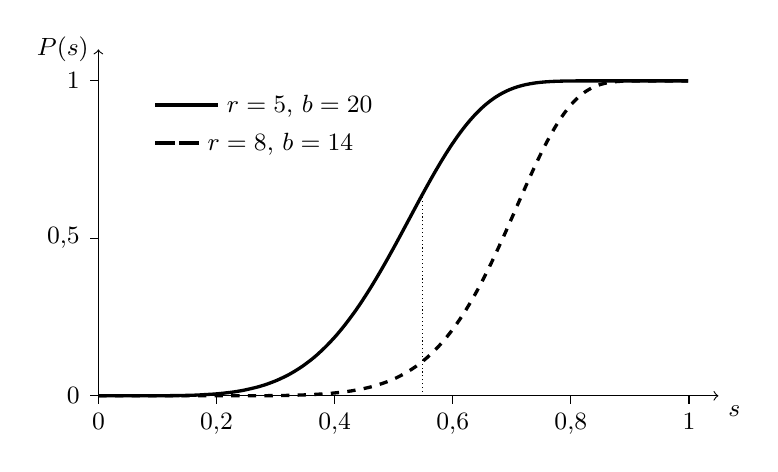
\begin{tikzpicture}[x=7.5cm,y=4cm,font=\small]
  \draw[->] (0,0)--(1.05,0) node[below right] {$s$};
  \draw[->] (0,0)--(0,1.1) node[left] {$P(s)$};
  \foreach \t in {0,0.2,0.4,0.6,0.8,1} \draw (\t,0)--(\t,-0.025) node[below] {\pgfmathprintnumber[use comma]{\t}};
  \foreach \t in {0,0.5,1} \draw (0,\t)--(-0.015,\t) node[left] {\pgfmathprintnumber[use comma]{\t}};
  \draw[very thick,domain=0:1,samples=120,smooth] plot (\x,{1-(1-\x^5)^20});
  \draw[very thick,dashed,domain=0:1,samples=120,smooth] plot (\x,{1-(1-\x^8)^14});
  \draw[densely dotted] (0.549,0)--(0.549,0.64);
  \node[anchor=west] at (0.08,0.92) {\rule[2pt]{8mm}{1.2pt}\ $r=5$, $b=20$};
  \node[anchor=west] at (0.08,0.80) {\rule[2pt]{2.5mm}{1.2pt}\,\rule[2pt]{2.5mm}{1.2pt}\ $r=8$, $b=14$};
\end{tikzpicture}
\caption{Curva en S de la \cref{prop:curva-s} para $(r,b)=(5,20)$ (continua; la línea punteada marca $(1/b)^{1/r}\approx 0{,}549$) y para la configuración de FineWeb, $(r,b)=(8,14)$ (discontinua).}
\label{fig:curva-s}
\end{figure}

\begin{ejemplo}[FineWeb]\label{ej:fineweb}
FineWeb calcula $112$ minhash sobre los $5$-gramas de palabras de cada documento y los agrupa en $b=14$ bandas de $r=8$~\cite[§3.4]{fineweb}. Para un par con $s=0{,}75$, $s^{8}=0{,}1001$ y $P=1-0{,}8999^{14}=0{,}772$, el valor del orden del $77\,\%$ que declara el artículo. La inflexión está en $s^{*}=(7/111)^{1/8}=0{,}708$. Los autores observaron además que deduplicar cada volcado por separado funcionaba mejor que deduplicar los $96$ volcados conjuntamente, que eliminaba hasta el $90\,\%$ de los datos antiguos.
\end{ejemplo}

\begin{lecturas}
\item Leskovec, Rajaraman y Ullman~\cite{mmds}, cap.~3 «Finding Similar Items», §3.1 a §3.4.
\item Stanford CS246~\cite{cs246}, clases «Locality-Sensitive Hashing~I» y «Locality-Sensitive Hashing~II».
\item Stanford CS336~\cite{cs336a4}, práctica~4, §3 «Deduplication» (problemas \texttt{exact\_deduplication} y \texttt{minhash\_deduplication}).
\item Broder~\cite{broder}, artículo original de MinHash.
\item Lee \emph{et al.}~\cite{lee}, efecto de la deduplicación sobre la memorización.
\end{lecturas}

\section*{Ejercicios del tema 2}
\addcontentsline{toc}{section}{Ejercicios del tema 2}

\begin{ejercicio}{1}{eje:2-porque}
¿Por qué un corpus con muchos duplicados es peor que uno deduplicado del mismo tamaño en tokens? Dé dos razones y un caso límite que las ilustre.
\end{ejercicio}

\begin{ejercicio}{1}{eje:2-conjuntos}
Calcule la similitud de Jaccard de cada par de conjuntos entre $S_1=\{a,b,c,d\}$, $S_2=\{b,c,e\}$ y $S_3=\{a,c,e,f\}$. ¿Qué par es el más parecido?
\fuente{adaptado de Leskovec, Rajaraman y Ullman~\cite{mmds}, cap.~3, ejercicio~3.1.1 (conjuntos modificados).}
\end{ejercicio}

\begin{ejercicio}{2}{eje:2-luna}
Calcule la similitud de Jaccard con $2$-shingles entre «la luna brilla sobre el mar» y «la luna brilla sobre el río». Explique por qué el resultado debe ser menor que $4/5$.
\end{ejercicio}

\begin{ejercicio}{2}{eje:2-firmas}
El universo es $\{0,1,2,3,4,5\}$, con $S_1=\{0,2,5\}$, $S_2=\{1,2,3\}$ y $S_3=\{0,3,5\}$. Se usan $h_1(x)=(x+1)\bmod 6$, $h_2(x)=(5x+1)\bmod 6$ y $h_3(x)=(2x+3)\bmod 6$. (a) ¿Cuáles de ellas son permutaciones del universo? (b) Calcule la firma MinHash de cada conjunto. (c) Compare la similitud estimada con la real para cada par.
\fuente{adaptado de Leskovec, Rajaraman y Ullman~\cite{mmds}, cap.~3, ejercicio~3.3.3 (conjuntos y funciones modificados).}
\end{ejercicio}

\begin{ejercicio}{2}{eje:2-lsh}
En un LSH con $r=4$ filas y $b=25$ bandas, calcule la probabilidad de que dos documentos sean candidatos si $s=0{,}3$ y si $s=0{,}85$. Calcule el umbral aproximado $(1/b)^{1/r}$ y el punto de inflexión exacto de la \cref{prop:curva-s}.
\end{ejercicio}

\begin{ejercicio}{2}{eje:2-curvas}
Para $(r,b)=(3,10)$, $(6,20)$ y $(5,50)$: (a) calcule $P(s)$ en $s=0{,}2$, $0{,}5$ y $0{,}8$; (b) calcule el valor exacto $s_{1/2}$ en que $P=1/2$ y compárelo con la aproximación $(1/b)^{1/r}$.
\fuente{adaptado de Leskovec, Rajaraman y Ullman~\cite{mmds}, cap.~3, ejercicios~3.4.1 y~3.4.2.}
\end{ejercicio}

\begin{ejercicio}{3}{eje:2-varianza}
(a) Demuestre que, para todo $J\in[0,1]$, la desviación típica del estimador del \cref{cor:estimador} es a lo sumo $1/(2\sqrt n)$. (b) Halle el menor $n$ que garantiza una desviación típica no mayor que $0{,}05$ para cualquier par de documentos, y el menor que la garantiza para pares con $J=0{,}8$. (c) Use la desigualdad de Chebyshev para acotar $\PP(\abs{\hat J-J}\ge 0{,}1)$ con $n=100$.
\end{ejercicio}
